\documentclass[10pt]{book} %,openbib


\usepackage[utf8x]{inputenc}
\usepackage{amsmath, amsfonts, mathrsfs, textcomp,amssymb,natbib,bbm,natbib}
\usepackage{multicol}
\usepackage{graphicx}

\title{Reproductive Allocation Calculations}
\author{K. Abramowicz, E. Wenk, D. Falster}
\date{\today}

\setlength{\textwidth}{151mm}\topmargin 7mm \textheight 210mm
\headheight 0mm \headsep 10mm \footskip 15mm \textwidth 151mm
\oddsidemargin 6.3mm \evensidemargin 6.3mm \marginparwidth 20mm


\begin{document}
\maketitle
\chapter{Software description}
\section{Purpose of software}
The goal of the code is to:
\begin{itemize}
\item Estimate reproductive investment from census data
\item Estimate growth investment
\item Determin Reproductive Allocation schedules for 14 species.
\end{itemize}
\section{Structure of Software}
\begin{center}
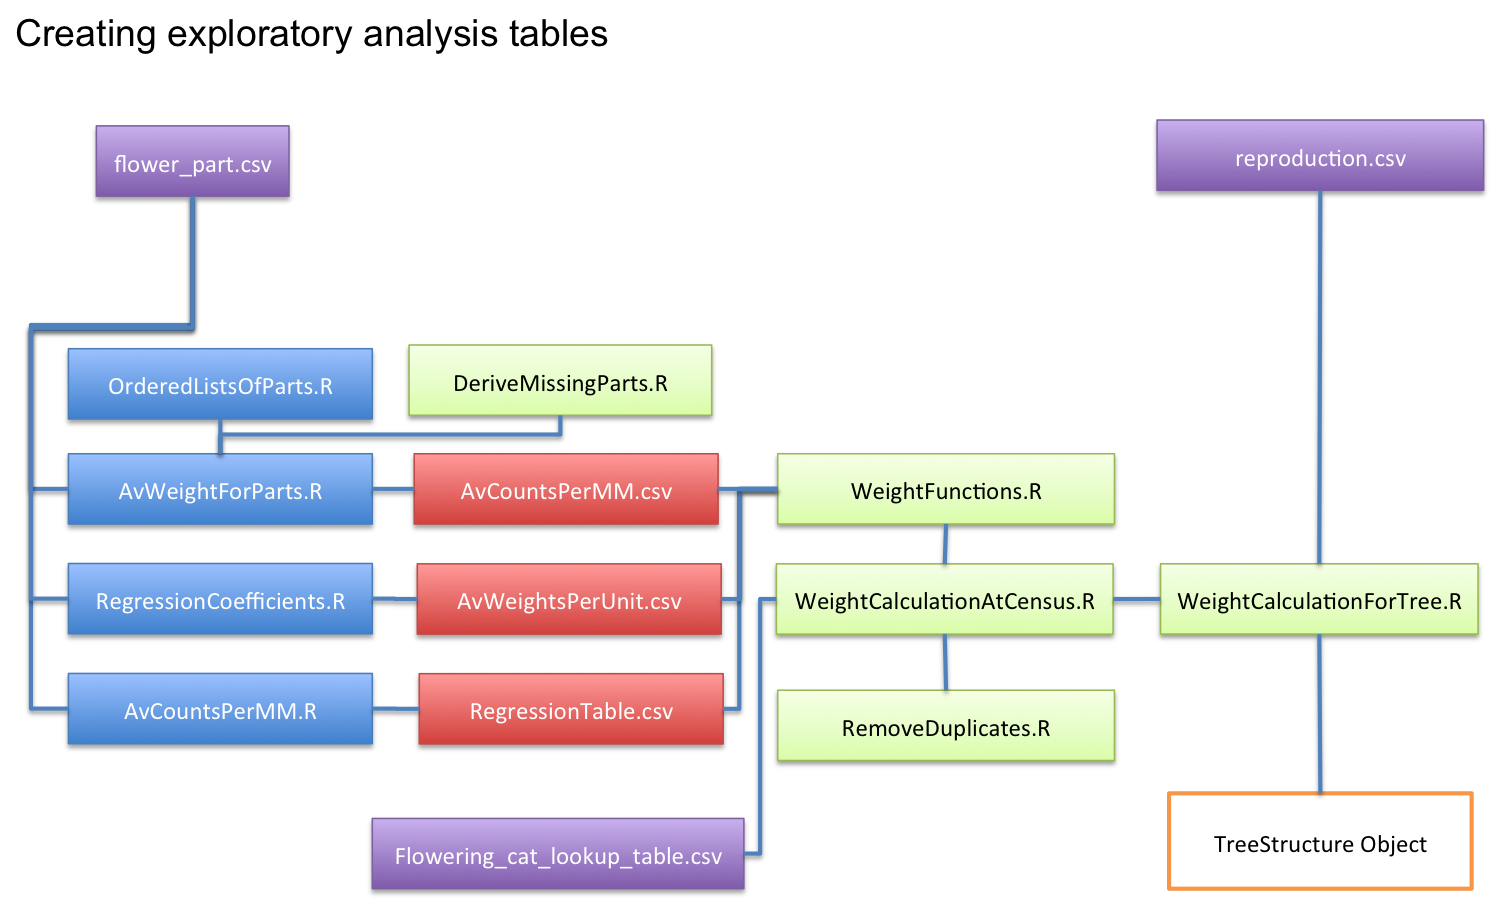
\includegraphics[width=0.75\linewidth]{images/Flow1.png}\\
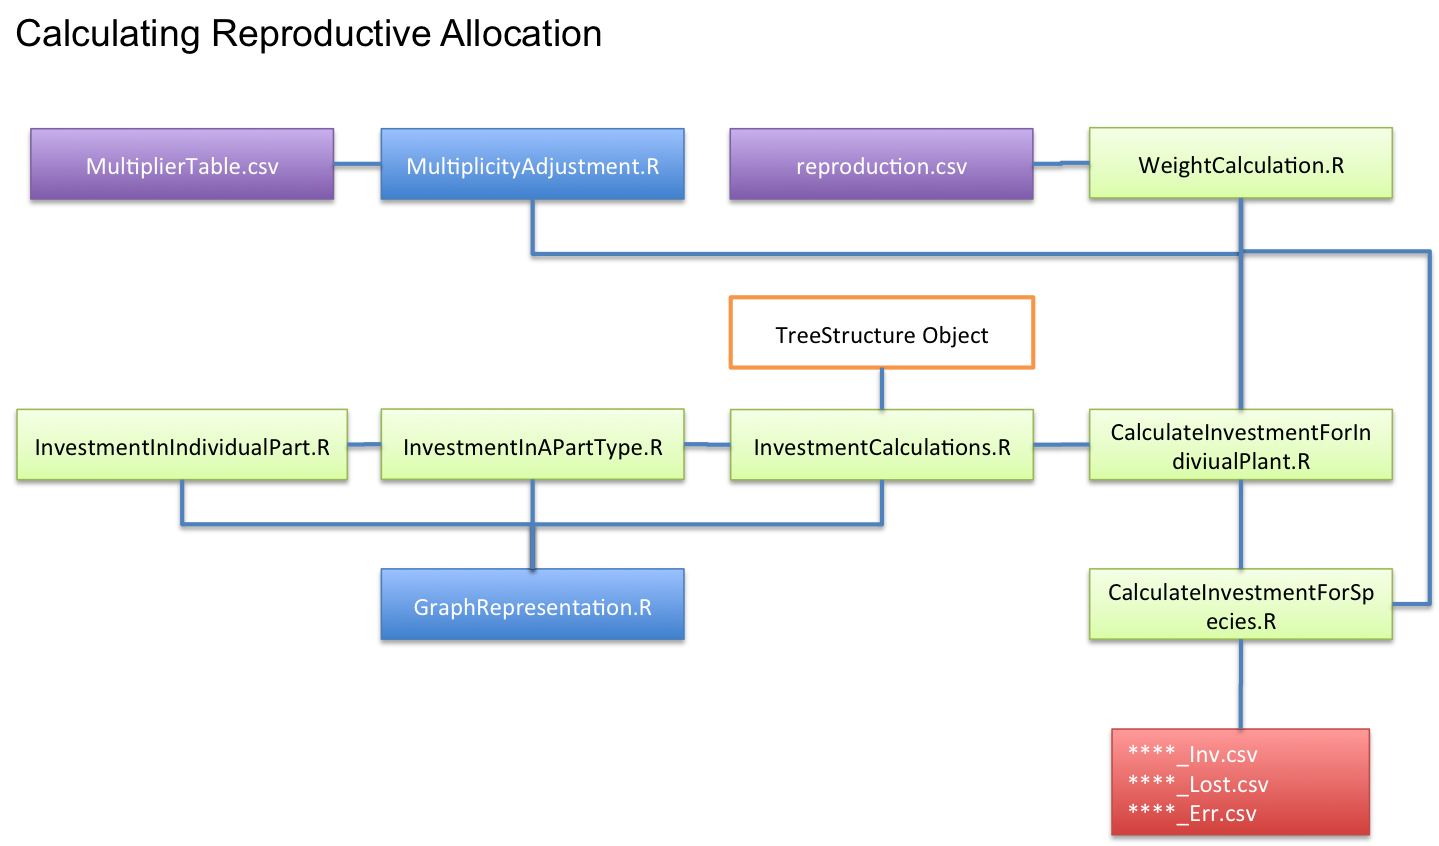
\includegraphics[width=0.75\linewidth]{images/Flow2.png}\\
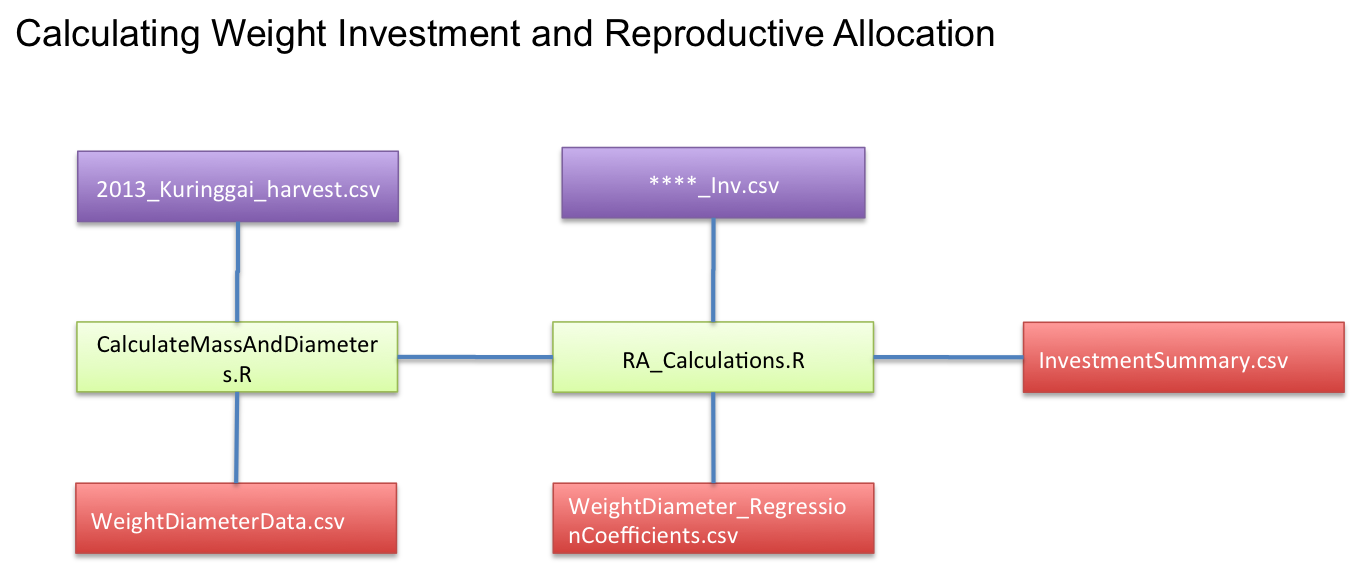
\includegraphics[width=0.75\linewidth]{images/Flow3.png}
\end{center}

\section{Listing of files}
\begin{itemize}
\item Data Files
\begin{itemize}
\item \texttt{flower\_parts.csv} File containing measurements of weight, length, and dimensions for given species. The file is used to obtain the average weights of plant parts based on the count, length and dimension measurements of individual species at given times.
\item \texttt{reproduction.csv} File containing information about counts, lengths and dimensions (not weights) for individuals at different censuses.
\item \texttt{2013\_Kuringgai\_harvest.csv} File containing information sbout diameters and weight for the sampled trees.
\item \texttt{Flowering\_cat\_lookup\_table.csv} File containing table describing the allowed parts of plants and the way they are measured.
\item \texttt{MultiplierTable.csv} File containing table describing the multiplicity of possible seed per plan part.
\end{itemize}
\item{R-functions' files}
\begin{itemize}
\item \texttt{WeightFunctions.R} - converts counts, lengths and dimensions to weights
\item \texttt{WeightCalculationAtCansus.R} - calculates weight of tree parts
\item \texttt{RemoveDumplicates.R} - merges multiple entries for the same tree parts
\item \texttt{DeriveMissingParts.R} - For particular species no measurements are provided/possible and they are being imputed with the values calculated by the script above.
\item \texttt{WeightCalculationsForTree.R} - calculates of weight dynamics for a tree along censuses
\item \texttt{InvestmentCalculations.R} - determines of investments of the plant along all censuses given a weight tree structure object
\item \texttt{InvestmentInAPartType.R} - calculates the investment in creation of a given type element at given census
\item \texttt{InvestmentInIndividualPart} - calculates the investment in creation of an \textbf{individual} of a given type at given census
\end{itemize}
\item{R-scripts}
\begin{itemize}
\item \texttt{AvWeightForParts.R} - calculates the average weights for the parts included in the {flower\_parts.csv} file for a given species.
\item \texttt{AvCountsPerMM.R} - calculates the average density of counts per mm for a given species. Saves results in AvCountsPerMM.csv
\item \texttt{RegressionCoefficients.R} - Script determining the regression coefficients that are use to obtain weights of elements from their dimensions.
\item \texttt{GraphRepresentation.R} - Script containing the structure for each specie which describes part names, their progression, and carbon flow.
\item \texttt{OrderedListsOfParts.R} - Script containing the ordered part names. Used for construction of this document.
\item \texttt{RedoDocument.R} - Short script calling all functions which produce tables and plots used in this document.
\item \texttt{CalculateMassAndDiameter.R} -script calculating and saving masses and diameters for the individual plants (using data in \texttt{2013\_Kuringgai\_harvest.csv})
\item \texttt{RA\_Calculations.R} - script reading reproductive investment, growth investment and calculating total investment and RA.
\end{itemize}
\item{Plotting functions}
\begin{itemize}
\item \texttt{Plot\_RAs} Function that plots and saves in a pdf RA for all the species on one plot.
\item \texttt{PlotIndividual\_RA} Function that for each species creates a 3 panel plot with reproductive investment, growth investment and RA.
\end{itemize}
\item Libraries used
\begin{itemize}
\item \texttt{igraph} used for representing and manipulating plant graphs.
\item \texttt{stringr} used for some string manipulations.
\item \texttt{colorspace} used for defining HCL colours for plotting RAs.
\end{itemize}
\end{itemize}

\newpage
%
%
% Individual functions
%
%
\section{Individual Functions Description}
\subsection*{WeightFromCount (in WeightFunctions.R)}
Given the count, species type and plant part the function returns a vector that contains the weight of each plant part. \\
Input parameters:
\begin{itemize}
\item \texttt{count}  integer describing number of observed plant parts
\item \texttt{species} character string defining the name of the species (as used in \texttt{flower\_part.csv}) file
\item \texttt{part} character sting corresponding to the name of the plant part
\end{itemize}
Output parameters:
\begin{itemize}
\item \texttt{w}  vector of length \texttt{count} with weight of the plant part at each position.
\end{itemize}

\subsection*{WeightFromLength (in WeightFunctions.R)}
Given the length of a body par, species type and plant part the function returns a vector that contains the weight of each plant part. The function uses the species specific relationship to estimate the count corresponding to the observed length. \\
Input parameters:
\begin{itemize}
\item \texttt{length}  double describing the length of observed plant parts
\item \texttt{species} character string defining the name of the species (as used in \texttt{flower\_part.csv}) file
\item \texttt{part} character sting corresponding to the name of the plant part
\end{itemize}
Output parameters:
\begin{itemize}
\item \texttt{w}  vector with weight of the plant part at each position. The size of the vector is estimated using allometric relationship.
\end{itemize}

\subsection*{WeightCalculationsAtCensus}
Given the census data from the measurement Excel spreadsheet the function creates a list which contains information about all existing parts, their counts, and weights.
\\
Input parameters:
\begin{itemize}
\item \texttt{C}  Data from a given census about an individual tree
\end{itemize}
Output parameters:
\begin{itemize}
\item \texttt{C\_list}   A list which elements are list that contain fields: \texttt{type} -part name, \texttt{m.type} - measurement type (count, length), \texttt{count} - number of such parts, \texttt{weight} - vector of weight for each part.
\end{itemize}

\subsection*{RemoveDuplicates}
Checks the list describing tree at a given census and merges multiple fields for the same tree part.
\\
Input parameters:
\begin{itemize}
\item \texttt{C}  List with the structure of output of \texttt{MeasurmentsToWeight} function.
\end{itemize}
Output parameters:
\begin{itemize}
\item \texttt{C\_new}  The same list with the fields for the same tree part merged. If there were two measurement types used for a given part the \texttt{m.type} is changed to \texttt{mixed}.
\end{itemize}


\subsection*{WeightCalculationsForTree}
Given the information about particular individual tree the functions returns a list representing the growth development of the tree.
\\
Input parameters:
\begin{itemize}
\item \texttt{Tree}  Rows of data.frame in  \texttt{reproduction.csv} corresponding to  an individual tree from all censuses
\end{itemize}
Output parameters:
\begin{itemize}
\item \texttt{TreeList}  A list which in the first element contains the tree id. The remaining 18 elements are 3 element lists with fields \texttt{pre.existing}, \texttt{new} and \texttt{total} describing the structure of the tree at each census. Each of the 3 lists is in the format corresponding to the result of \texttt{MeasurmentsToWeight} function.
\end{itemize}

\subsection*{AdjustForMultiplicity (in MultiplicityAdjustment.R)}
Function \texttt{AdjustForMultiplicity} together with its help functions (\texttt{AdjustForMultiplicity\_Census,AdjustForMultiplicity\_List}) that given Tree Structure adjust counts and weights to take into account number of seeds per fruit/flower etc.
Input parameters:
\begin{itemize}
\item \texttt{Tree}  Tree structure with weights and individual ID of a plant (result of WeightCalculationsForTree)
\end{itemize}
Input parameters:
\begin{itemize}
\item \texttt{Tree}  Tree structure with weights and individual ID of a plant (result of WeightCalculationsForTree), where counts are multiplied by multipliers and weights are divided.
\end{itemize}




\subsection*{InvestmentInIndividualPart}
Given element name, its weight, allowed progression and the list of possible existing predecessors the function returns the investment  that was made to grow the element from its previous form to the existing one.
Input parameters:
\begin{itemize}
\item \texttt{Element}  Name of element
\item \texttt{TreeList\_Pred}  Tree structure (similar to the result of WeightCalculcations function) with possible predecessors. Its length determine the time point at which we are now.
\item \texttt{Progression} Character vector defining the possible previous stages of the Element.
\item \texttt{El\_weight} Weight of the element.

\end{itemize}
Output parameter is a list containing 6 elements
\begin{itemize}
\item \texttt{TreeList\_Pred}  Updated list of possible predecessors with the used predecessor removed.
\item \texttt{Invest} Calculated investment (using the path from element to it's predecessor, incorporating the carbon flow in case of division)
\item \texttt{from} Selected predecessor's name
\item \texttt{to} The same as  \texttt{Element}
\item \texttt{Census} Information at which census the transition to Element has been observed.
\item \texttt{Count} 1.
\end{itemize}

\noindent \textbf{Function description:}
\begin{itemize}
\item Given the element, possible predecessor and history of development of the tree, the function performs a back search in history looking for matching Predecessor.
\item After finding Predecessor the investment is calculated. The investment is defined as the difference between the Element mass and the proportion of the mass of Predecessor. If the path from Predecessor to the Element does not have any accessory tissue the proportion will be 1. Otherwise the side allocation of the carbon to the accessory tissue is taken into consideration.
\item The predecessor is removed from the list of possible predecessors and the list is returned for further calculations.
\end{itemize}


\subsection*{InvestmentInAPartType}
Given part name, tree structure, allowed progression and the tree structure of possible existing predecessors the function returns the investment that was made to grow the plant part of a given type. It also calculates the investment in all newly created elements of a given type.
Input parameters:
\begin{itemize}
\item \texttt{TreeList}  Tree structure (like the result of WeightCalculcations function) containing information about the plant. The length of the list determine current time point.
\item \texttt{TreeList\_Pred}  Tree structure (like the result of WeightCalculcations function) with possible predecessors.
\item \texttt{Element}  Name of element
\item \texttt{Progression} Character vector defining the possible previous stages of the Element.
\end{itemize}
Output parameter is a list containing 2 elements
\begin{itemize}
\item \texttt{TreeList\_Pred}  Updated list of possible predecessors with the used predecessors removed.
\item \texttt{Invest} Data structure containing information about investment in creation/progression of all elements of a given type at a given time.
\end{itemize}

\noindent \textbf{Function description:}
\begin{itemize}
\item Function determines the census by calculating length of TreeList\_Pred.
\item First we check if there are new elements of given type at this time point. If yes, the investment in them is calculated as their weight.
\item The function checks if there are pre.existing elements of that type. If yes, it checks how many they are and use function CalculateIndividualInvestment to find the investment made in them attaining the stat.
\item \textit{OBS!} Exception is made if at the first census we have a part that is pre.existing. It's mass is not to be counted as new since it was created outside the monitoring period, however, the information about it needs to be included as in later censuses it might develop resulting in carbon investment.
\end{itemize}

\subsection*{InvestmentCalculations}
Given a tree structure along all censuses the history of investment is calculated.
Input parameters:
\begin{itemize}
\item \texttt{TreeList}  Tree structure (the result of WeightCalculcations function) containing information about the plant.
\end{itemize}
Output parameter:
\begin{itemize}
\item \texttt{Inv} Data frame containing information about investment in creation/progression of specific parts along all censuses.
\item \texttt{Lost} Data frame containing information about lost parts.
\item \texttt{Error} Data frame containing information about possible errors (missing predecessors to preexisting species).
\end{itemize}

\noindent \textbf{Function description:}
\begin{itemize}
\item First the structure of the specie is determined and number of main paths is determined. Then for each of the main paths:
\begin{itemize}
\item We determine the main progression line, and go backwards census by census along all elements in the main progression lines calculating the investment.
If the line includes "x-or" parts (mostly aborted fruits,flowers) calculation  along this lines is made as well.
\item After calculating main and "x-or" lines the list of possible predecessors is reset to all values and separate carbon investment is performed for each of the auxiliary tissue type.
\end{itemize}
\end{itemize}

\subsection*{CalculateInvestmentForIndividualPlane}
Given the name (tag\_ID) of the individual plant, calculations of reproductive investment are performed.
Input parameters:
\begin{itemize}
\item \texttt{individual}  String corresponding to tree ID in the reproduction spreadsheet
\end{itemize}
Output parameter is a list including 3 data frames
\begin{itemize}
\item \texttt{Inv} Data frame containing information about investment in creation/progression of specific parts along all censuses.
\item \texttt{Lost} Data frame containing information about lost parts.
\item \texttt{Error} Data frame containing information about possible errors (missing predecessors to preexisting element).
\end{itemize}

\subsection*{CalculateInvestmentForSpecies}
A wrapper around function \texttt{CalculateInvestmentForIndividualPlane} that given string specifying specie name calculates the investment for all individuals of the species and saves the result in csv files.
Input parameters:
\begin{itemize}
\item \texttt{TreeList}  Tree structure (the result of WeightCalculcations function) containing information about the plant.
\end{itemize}
The function does not return anything, however it saves 3 files(\texttt{****} stands for species name):
\begin{itemize}
\item \texttt{****\_Inv} Information about investment in creation/progression of specific parts along all censuses for all the individuals.
\item \texttt{****\_Lost} Information about lost parts for all individuals.
\item \texttt{****\_Error} Information about possible errors (missing predecessors to preexisting element).
\end{itemize}


\subsection{GraphRepresentation}

Script \texttt{GraphRepresentatio.R} contains the definitions of the graph structures defining plant development. This structures mimic to a large extent the plant maps.
Each specie is represented by \texttt{igraph} object and a data frame \texttt{Paths} defining main progression lines for the species.

The graph object consist of:
\begin{itemize}
\item Vertices with name being a part name. Each vertex is also coloured. The distinct progression lines have distinct colour. Moreover the final stages of the accessory tissues have colour with a number larger by 1 from the main path they belong to.
\item Edges that connect the subsequent parts on the map. Each edge has a weight attribute defining how much of the carbon allocated the predecessor is being used for ancestor creation. If there are no accessory tissues created at this point of progression weight will be 1. If there is more than one ancestor the weights are set as the proportion of the ancestor mass to the sum of all ancestors. This is done at that point manually and needs to be adjusted if any new data will be collected.
\end{itemize}
An example of the graph for CEOR species is presented in Figure 1.1.


\begin{figure}[htb]
\begin{center}
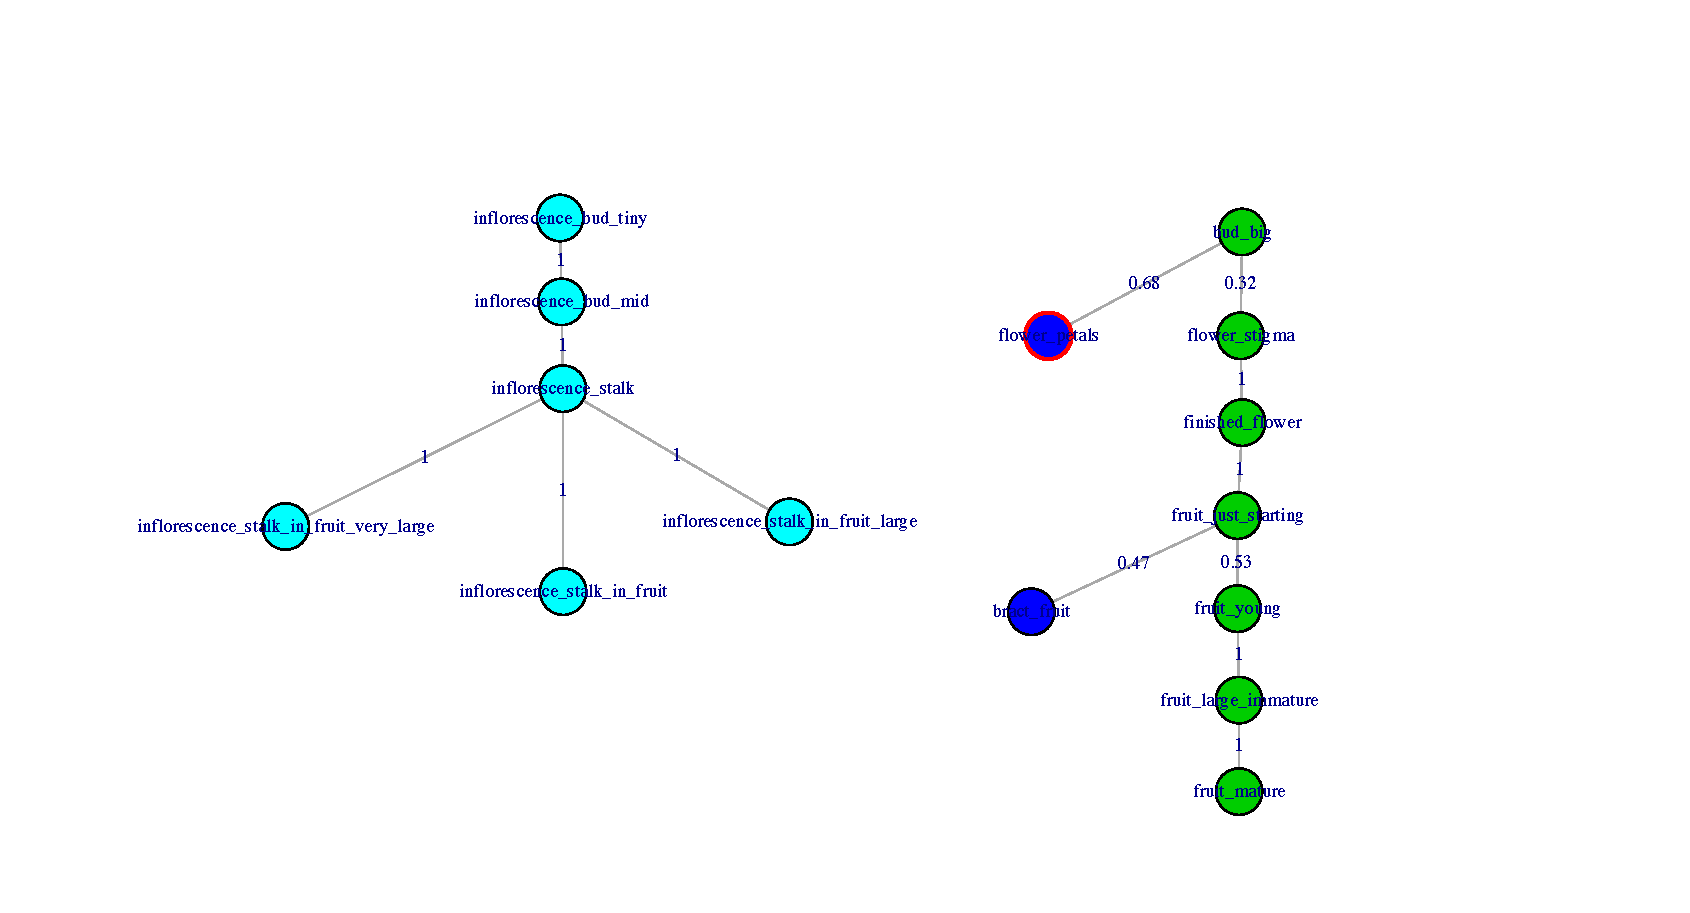
\includegraphics[width=6in]{images/PlantGraph.pdf}
\end{center}
\caption{Graphical presentation of the \texttt{igraph} tree structure of plant map for COER.}
\end{figure}


\chapter{Species Average Weight Summary}
\newpage
\footnotesize



\clearpage
\newpage
\section{BAER}
\begin{multicols}{2}
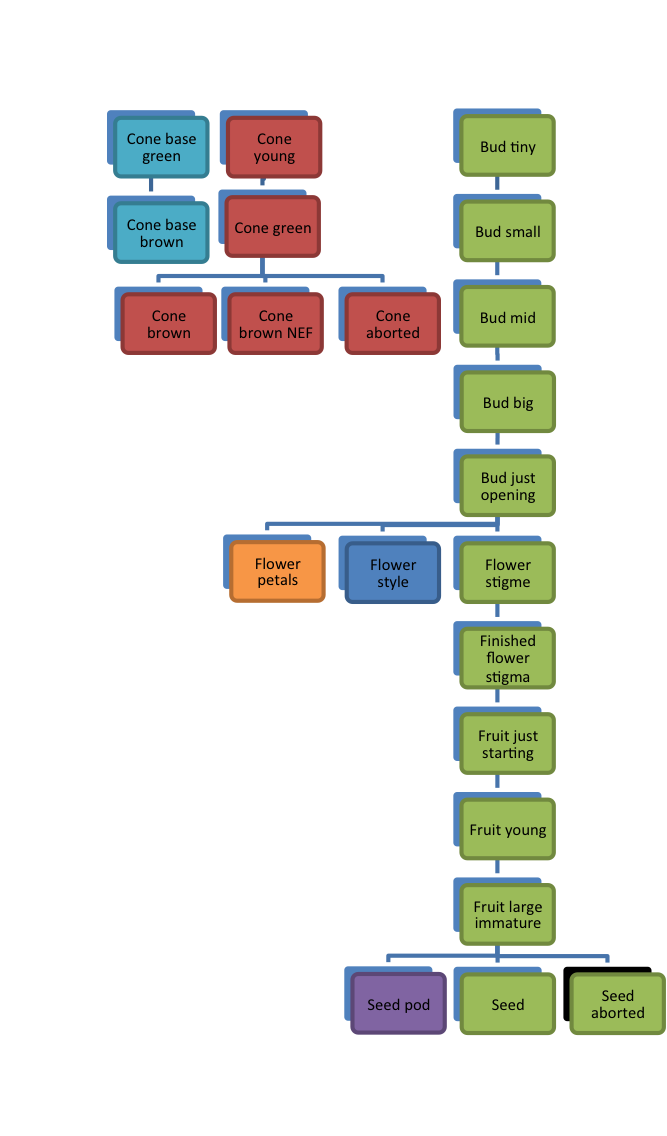
\includegraphics[width=3in]{images/BAER.png}
\vfill
\columnbreak
\input{tables/BAER.tex}
\end{multicols}



\clearpage
\newpage
\section{BOLE}
\begin{multicols}{2}
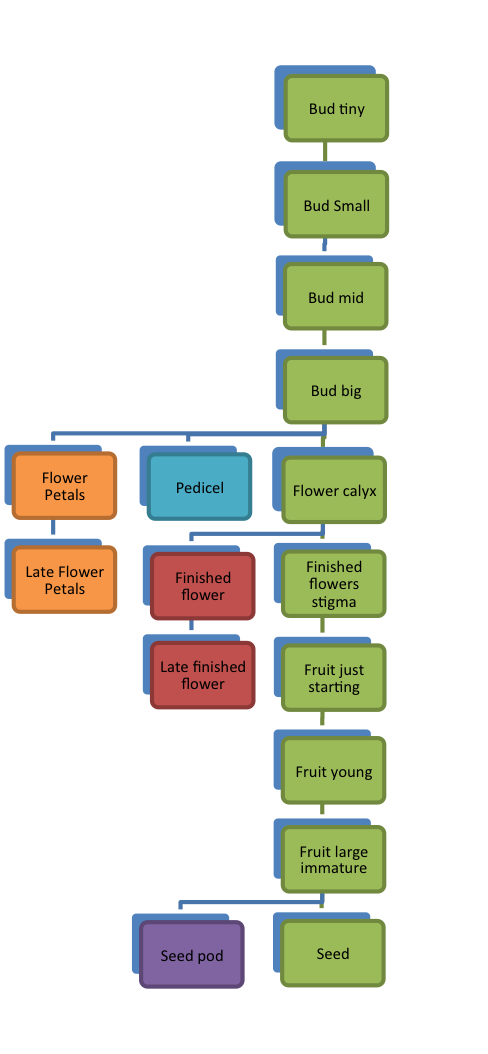
\includegraphics[width=3in]{images/BOLE.png}
\vfill
\columnbreak
\input{tables/BOLE.tex}
\end{multicols}


\clearpage
\newpage



\section{COER}
\begin{multicols}{2}
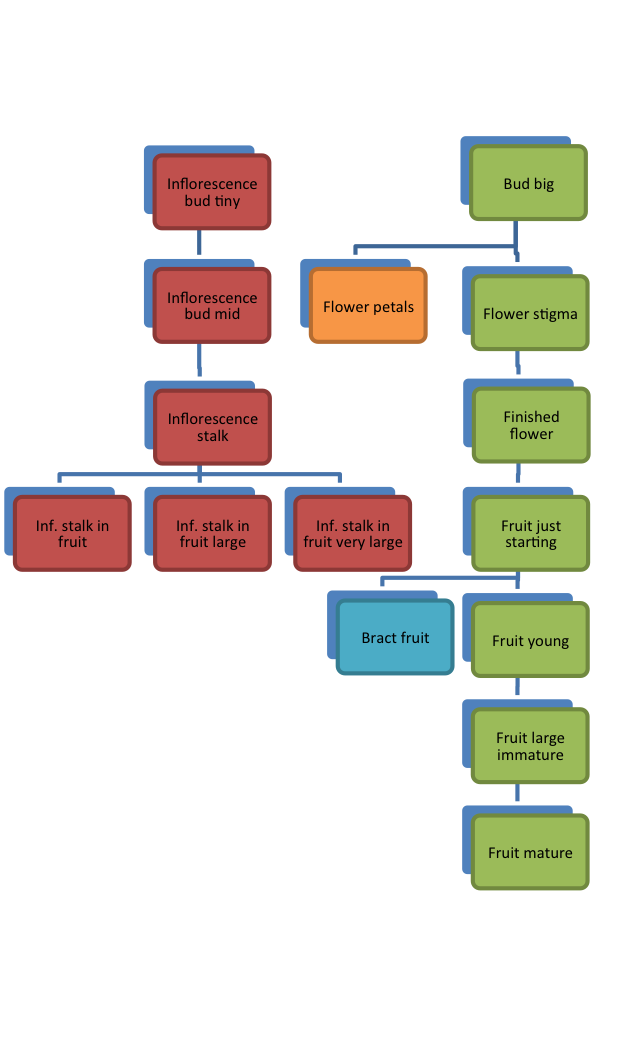
\includegraphics[width=2.7in]{images/COER.png}
\vfill
\columnbreak
\input{tables/COER.tex}
\end{multicols}

\clearpage
\newpage


\section{EPMI}
\begin{multicols}{2}
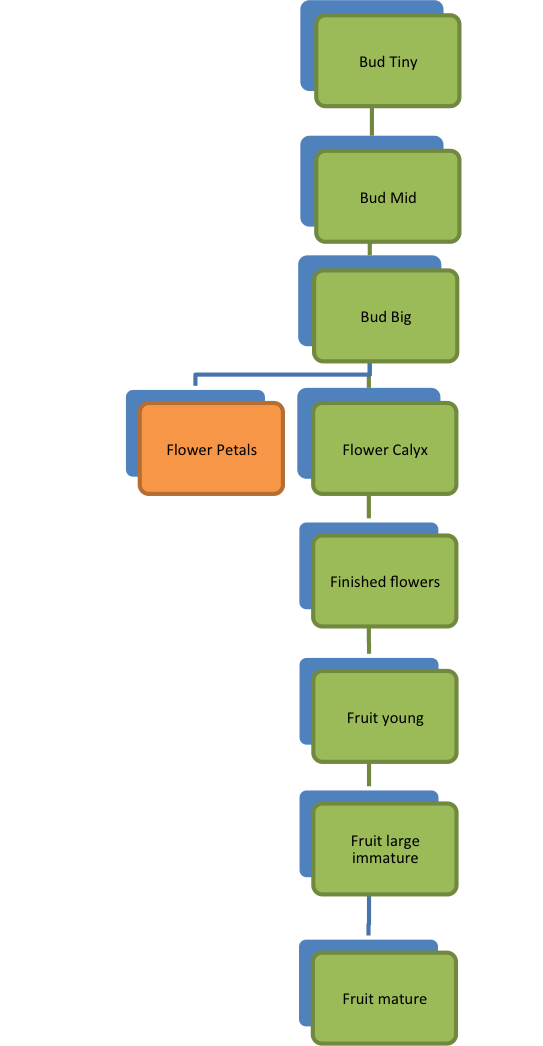
\includegraphics[width=2.5in]{images/EPMI.png}
\vfill
\columnbreak
\input{tables/EPMI.tex}
\end{multicols}

\clearpage
\newpage


\section{GRBU}
\begin{multicols}{2}
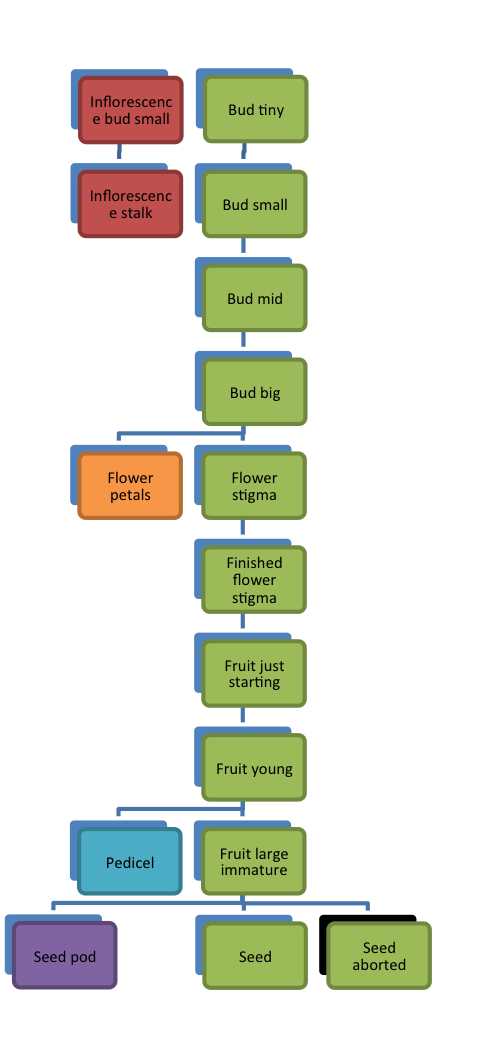
\includegraphics[width=3in]{images/GRBU.png}
\vfill
\columnbreak

\input{tables/GRBU.tex}\\

\end{multicols}

\clearpage
\newpage

\section{GRSP}
\begin{multicols}{2}
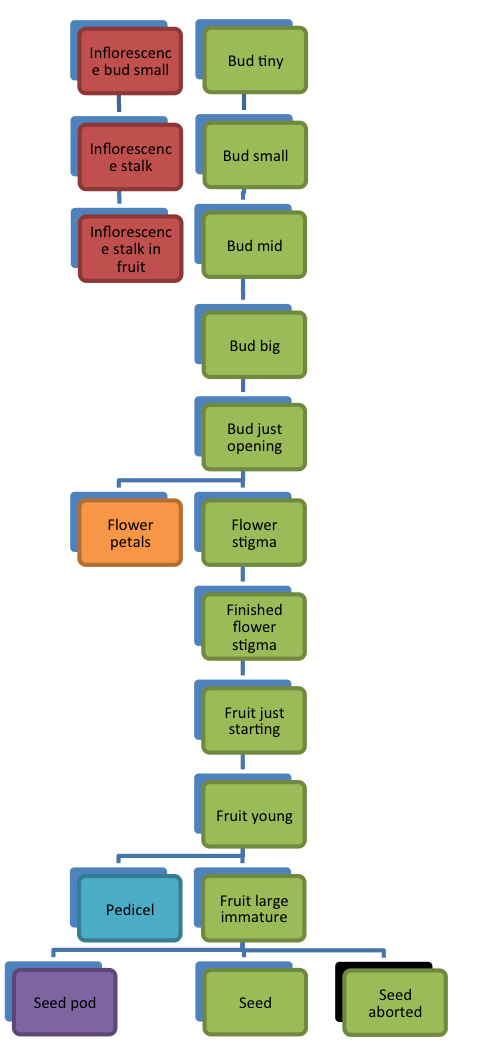
\includegraphics[width=3in]{images/GRSP.png}
\vfill
\columnbreak

\input{tables/GRSP.tex}

\end{multicols}




\clearpage
\newpage
\section{HATE}
\begin{multicols}{2}
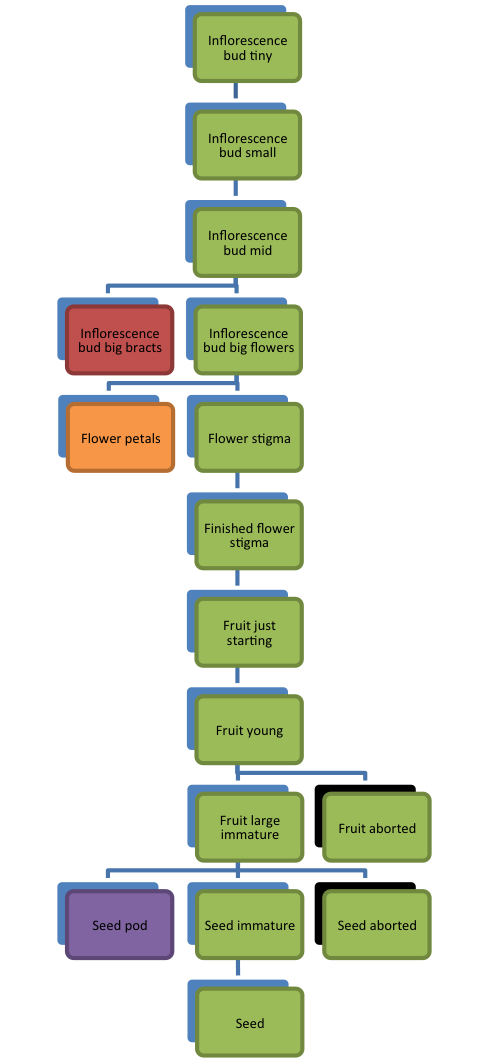
\includegraphics[width=3in]{images/HATE.png}
\vfill
\columnbreak
\input{tables/HATE.tex}

\end{multicols}

\clearpage
\newpage



\section{HEPU}
\begin{multicols}{2}
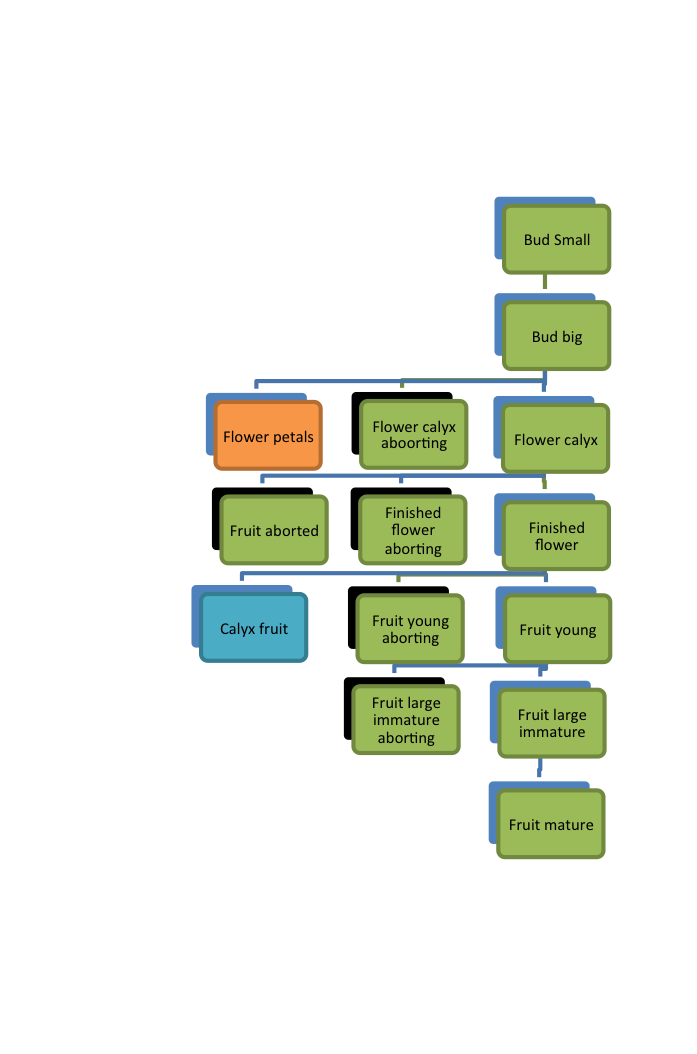
\includegraphics[width=3in]{images/HEPU.png}
\vfill
\columnbreak
\input{tables/HEPU.tex}
\end{multicols}

\clearpage
\newpage

\section{LEES}
\begin{multicols}{2}
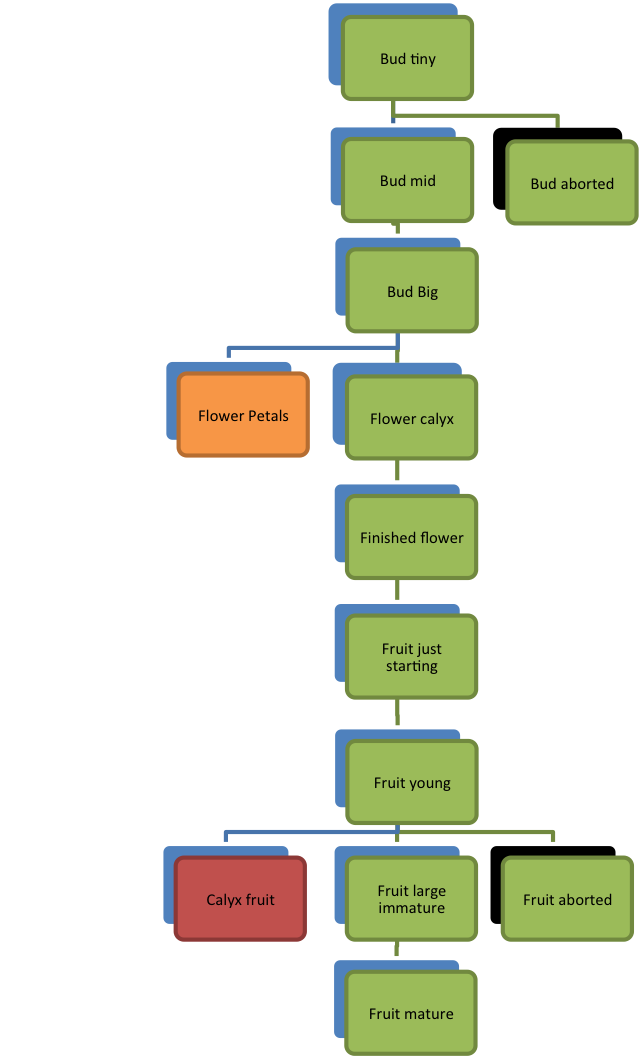
\includegraphics[width=3in]{images/LEES.png}
\vfill
\columnbreak
%%%%
\input{tables/LEES.tex}
%%%%%
\\
\end{multicols}
\clearpage
\newpage


\section{PELA}
\begin{multicols}{2}
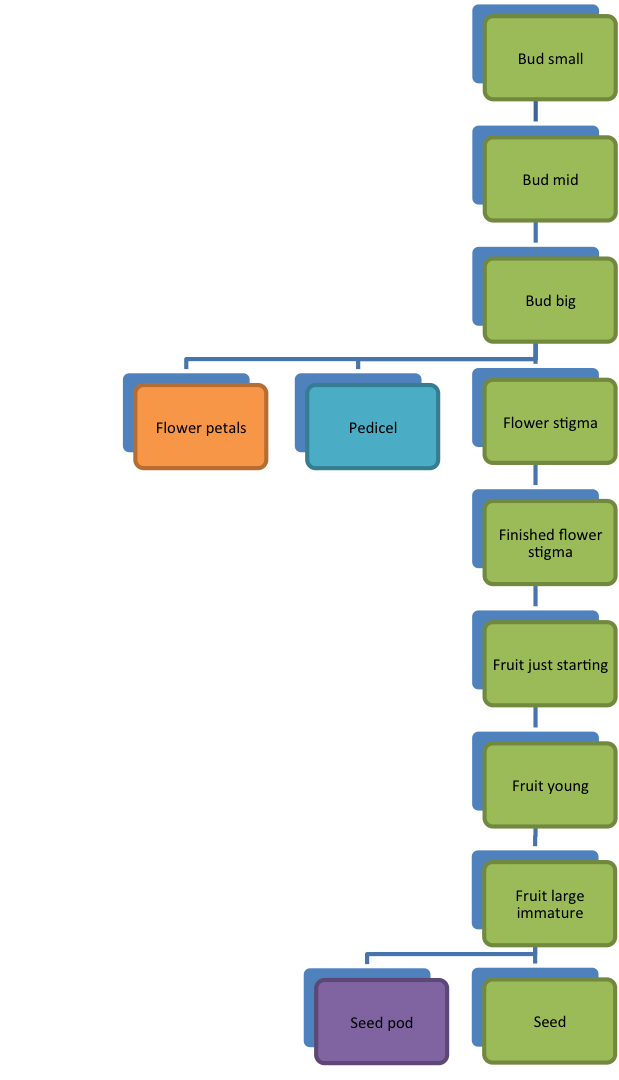
\includegraphics[width=2.8in]{images/PELA.png}
\vfill
\columnbreak
\input{tables/PELA.tex}
\end{multicols}



\clearpage
\newpage
\section{PEPU}
\begin{multicols}{2}
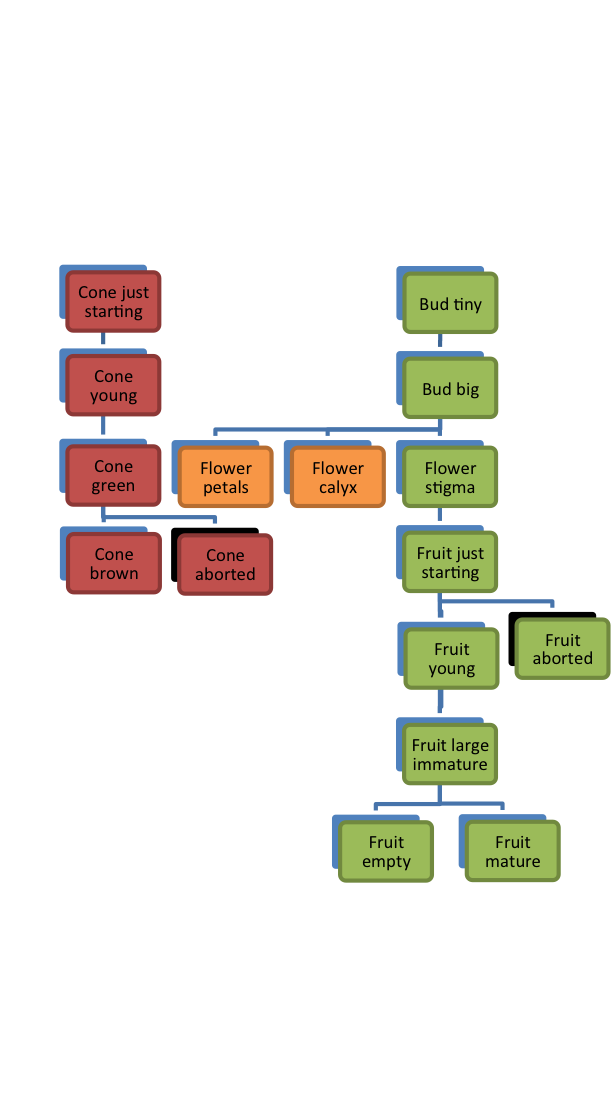
\includegraphics[width=2.7in]{images/PEPU.png}
\vfill
\columnbreak
\input{tables/PEPU.tex}
\end{multicols}
\clearpage
\newpage


\clearpage
\newpage
\section{PHPH}
\begin{multicols}{2}
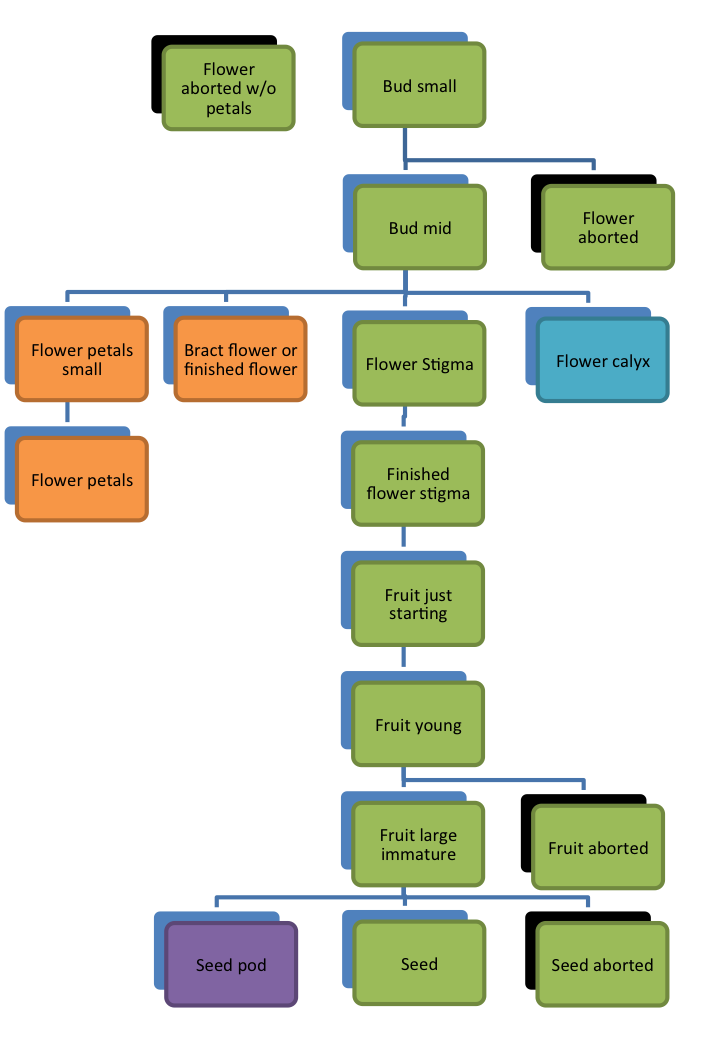
\includegraphics[width=3in]{images/PHPH.png}
\vfill
\columnbreak
\input{tables/PHPH.tex}
\end{multicols}



\clearpage
\newpage
\section{PILI}
\begin{multicols}{2}
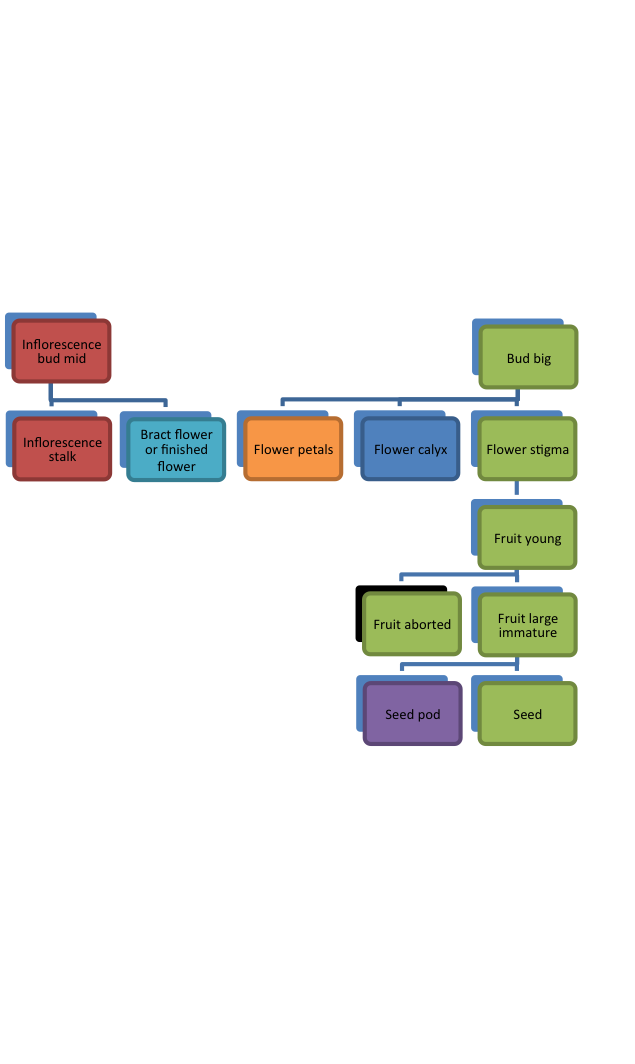
\includegraphics[width=2.7in]{images/PILI.png}
\vfill
\columnbreak
\input{tables/PILI.tex}
\end{multicols}





\clearpage
\newpage
\section{PUTU}
\begin{multicols}{2}
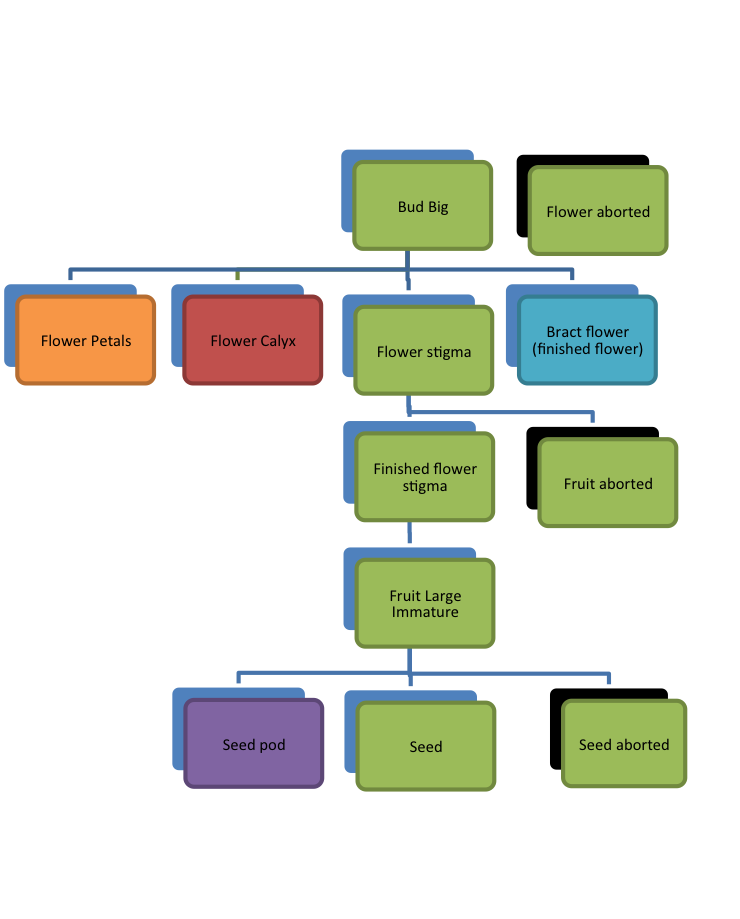
\includegraphics[width=2.5in]{images/PUTU.png}
\vfill
\columnbreak
\input{tables/PUTU.tex}
\end{multicols}




\chapter{Additional preliminary calculations}

\section{Average count/length values}


\begin{figure}[h!]
\begin{center}
\input{tables/AvCountsPerMM.tex}
\end{center}
\caption{Table summarising the average number of elements per mm. To be used for calculations of mass based on the length for conversion to counts.}
\end{figure}


% TODO: Include these plots
% \section{Regression Fits and Coefficients}
% \subsection*{GRBU}
% \begin{center}
% \includegraphics[width=2.7in]{figures/GRBU_fruit_large_immature.pdf}
% \includegraphics[width=2.7in]{figures/GRBU_seed_pod.pdf}
% \end{center}

% \subsection{GRSP}
% \begin{center}
% \includegraphics[width=2.7in]{figures/GRSP_fruit_large_immature.pdf}
% \includegraphics[width=2.7in]{figures/GRSP_seed_pod.pdf}
% \end{center}

% \subsection{PELA}
% \begin{center}
% \includegraphics[width=2.7in]{figures/PELA_fruit_large_immature.pdf}
% \includegraphics[width=2.7in]{figures/PELA_seed_pod.pdf}\\
% \includegraphics[width=2.7in]{figures/PELA_seed.pdf}
% \end{center}

% \subsection{BAER}
% \begin{center}
% \includegraphics[width=2.7in]{figures/BAER_cone_young.pdf}
% \includegraphics[width=2.7in]{figures/BAER_cone_green.pdf}\\
% \includegraphics[width=2.7in]{figures/BAER_cone_brown_no_expanded_follicles.pdf}
% \includegraphics[width=2.7in]{figures/BAER_cone_brown.pdf}\\
% \includegraphics[width=2.7in]{figures/BAER_cone_aborted.pdf}
% \includegraphics[width=2.7in]{figures/BAER_cone_base_green.pdf}\\
% \includegraphics[width=2.7in]{figures/BAER_cone_base_brown.pdf}
% \end{center}

% \subsection{PEPU}
% \begin{center}
% \includegraphics[width=2.7in]{figures/PEPU_cone_green.pdf}
% \includegraphics[width=2.7in]{figures/PEPU_cone_brown.pdf}\\
% \includegraphics[width=2.7in]{figures/PEPU_cone_aborted.pdf}
% \end{center}


\newpage
\subsection{Summary table for regression}
\begin{figure}[h!]
\begin{center}
\input{tables/RegressionTable.tex}
\end{center}
\caption{Table summarising the equations used to determine weights of individual plant parts by using their size.}
\end{figure}

\chapter{Preliminary results}
\section{Reproductive allocation results}
\subsection{Overview}
\includegraphics[width=1\linewidth]{figures/RA_comparison_age.pdf}
\includegraphics[width=1\linewidth]{figures/RA_comparison_diam.pdf}
\includegraphics[width=1\linewidth]{figures/RA_comparison_weight.pdf}
\clearpage

TODO:Add this material back in

\newpage
\section{Individual species}
\subsection{BAER}
\includegraphics[width=1\linewidth]{figures/RA_age_BAER.pdf}
\includegraphics[width=1\linewidth]{figures/RA_weight_diam_BAER.pdf}

\clearpage
\newpage
\subsection{BOLE}
\includegraphics[width=1\linewidth]{figures/RA_age_BOLE.pdf}
\includegraphics[width=1\linewidth]{figures/RA_weight_diam_BOLE.pdf}

\clearpage
\newpage
\subsection{COER}
\includegraphics[width=1\linewidth]{figures/RA_age_COER.pdf}
\includegraphics[width=1\linewidth]{figures/RA_weight_diam_COER.pdf}

\clearpage
\newpage
\subsection{EPMI}
\includegraphics[width=1\linewidth]{figures/RA_age_EPMI.pdf}
\includegraphics[width=1\linewidth]{figures/RA_weight_diam_EPMI.pdf}

\clearpage
\newpage
\subsection{GRBU}
\includegraphics[width=1\linewidth]{figures/RA_age_GRBU.pdf}
\includegraphics[width=1\linewidth]{figures/RA_weight_diam_GRBU.pdf}

\clearpage
\newpage
\subsection{GRSP}
\includegraphics[width=1\linewidth]{figures/RA_age_GRSP.pdf}
\includegraphics[width=1\linewidth]{figures/RA_weight_diam_GRSP.pdf}

\clearpage
\newpage
\subsection{HATE}
\includegraphics[width=1\linewidth]{figures/RA_age_HATE.pdf}
\includegraphics[width=1\linewidth]{figures/RA_weight_diam_HATE.pdf}

\clearpage
\newpage
\subsection{HEPU}
\includegraphics[width=1\linewidth]{figures/RA_age_HEPU.pdf}
\includegraphics[width=1\linewidth]{figures/RA_weight_diam_HEPU.pdf}

\clearpage
\newpage
\subsection{LEES}
\includegraphics[width=1\linewidth]{figures/RA_age_LEES.pdf}
\includegraphics[width=1\linewidth]{figures/RA_weight_diam_LEES.pdf}

\clearpage
\newpage
\subsection{PELA}
\includegraphics[width=1\linewidth]{figures/RA_age_PELA.pdf}
\includegraphics[width=1\linewidth]{figures/RA_weight_diam_PELA.pdf}

\clearpage
\newpage
\subsection{PEPU}
\includegraphics[width=1\linewidth]{figures/RA_age_PEPU.pdf}
\includegraphics[width=1\linewidth]{figures/RA_weight_diam_PEPU.pdf}

\clearpage
\newpage
\subsection{PHPH}
\includegraphics[width=1\linewidth]{figures/RA_age_PHPH.pdf}
\includegraphics[width=1\linewidth]{figures/RA_weight_diam_PHPH.pdf}

\clearpage
\newpage
\subsection{PILI}
\includegraphics[width=1\linewidth]{figures/RA_age_PILI.pdf}
\includegraphics[width=1\linewidth]{figures/RA_weight_diam_PILI.pdf}

\clearpage
\newpage
\subsection{PUTU}
\includegraphics[width=1\linewidth]{figures/RA_age_PUTU.pdf}
\includegraphics[width=1\linewidth]{figures/RA_weight_diam_PUTU.pdf}

% \newpage
% \section{Investment in Accessory Tissues}
% \subsection{Overview}
% \includegraphics[width=1\linewidth]{figures/IAT_Comparison.pdf}
% \clearpage
% \newpage
% \section{Individual species}
% \subsection{BAER}
% \includegraphics[width=1\linewidth]{figures/IAT_BAER.pdf}

% \subsection{BOLE}
% \includegraphics[width=1\linewidth]{figures/IAT_BOLE.pdf}

% \subsection{COER}
% \includegraphics[width=1\linewidth]{figures/IAT_COER.pdf}

% \subsection{EPMI}
% \includegraphics[width=1\linewidth]{figures/IAT_EPMI.pdf}

% \subsection{GRBU}
% \includegraphics[width=1\linewidth]{figures/IAT_GRBU.pdf}

% \subsection{GRSP}
% \includegraphics[width=1\linewidth]{figures/IAT_GRSP.pdf}

% \subsection{HATE}
% \includegraphics[width=1\linewidth]{figures/IAT_HATE.pdf}

% \subsection{HEPU}
% \includegraphics[width=1\linewidth]{figures/IAT_HEPU.pdf}

% \subsection{LEES}
% \includegraphics[width=1\linewidth]{figures/IAT_LEES.pdf}

% \subsection{PELA}
% \includegraphics[width=1\linewidth]{figures/IAT_PELA.pdf}

% \subsection{PEPU}
% \includegraphics[width=1\linewidth]{figures/IAT_PEPU.pdf}

% \subsection{PHPH}
% \includegraphics[width=1\linewidth]{figures/IAT_PHPH.pdf}

% \subsection{PILI}
% \includegraphics[width=1\linewidth]{figures/IAT_PILI.pdf}

% \subsection{PUTU}
% \includegraphics[width=1\linewidth]{figures/IAT_PUTU.pdf}







\end{document}

